\subsection{Initial experiments with KENN}
The goal of these experiments is to analyze how KENN behaves when involved in a FET task. When the framework has been introduced in section \ref{KENN}, we saw that it allows using different settings about clause weights (i.e., fixed values, learnable parameters). However, the best choice for this context needs to be discovered. The same goes for the KB modes, as several alternatives were proposed without knowing which one would be the most promising for our task. Given these premises, the analysis can be divided into two parts. The first part is constituted by some \textit{quantitative analysis} (section~\ref{quantitative_analysis}) and aims to study the impact of each configuration of KENN. The second part is called \textit{preactivations analysis} (section~\ref{preactivation_analysis}) and investigates what happens in the network at a lower level.

\subsubsection{Setup}
Both the baseline and KENN-based models used in these experiments follow the \textit{Setup A}. The tested configurations are obtained with the following parameters:
\begin{itemize}
    \item \textbf{KB modes:} Bottom Up, Top Down and Hybrid
    \item \textbf{initial clause weights:} 0.5, 1.0 and 2.0
    \item \textbf{fixed clause weights}
    \item \textbf{encoder:} DistilBERT with adapters
    \item \textbf{loss function:} Binary Cross-Entropy, with the weights of positive examples set to 1
\end{itemize}
Each KB mode is tested by varying the initial clause weight, counting a total of 9 KENN's configurations. Clause weights are set as non-learnable parameters to force KENN to treat them all equally during the enhancement process and to ensure the presence of KENN for all the training.

\subsubsection{Terminology}
The following terminology will be used during the analysis:
\begin{itemize}
    \item \textbf{F:} stands for \textit{Father} (i.e, supertype); used to indicate a type that corresponds to a father node in the hierarchical tree
    \item \textbf{S:} stands for \textit{Son} (i.e., subtype); used to indicate a type that corresponds to a child node in the hierarchical tree
    \item \textbf{pre-KENN state:} values of the preactivations provided to KENN as input
    \item \textbf{post-KENN state:} values of the preactivations after KENN (i.e., final output)
\end{itemize}
\textit{\textbf{Additional note:} in some circumstances we may say that the baseline model and the pre-KENN network are equivalent. To avoid misunderstanding, the term ``equivalent" is intended as identical architecture and initialization, excluding KENN's layer.}


\subsubsection{Quantitative analysis} \label{quantitative_analysis}
This is a high-level analysis based on the performance obtained by the models on the dev set during the training process. The involved studies will try to answer the following questions:
\begin{enumerate}
    \item \textbf{Effects of different clause weights:} how much does the weight of a clause affect the final predictions?
    \item \textbf{Effects of each KB mode:} is there a winning strategy to define clauses that brings more benefits than the others? does the winning strategy perform better than the baseline?
    \item \textbf{Metrics per type:} is there a KB mode that enhances the performance on certain types?
\end{enumerate}

\subsubsection{Preactivations analysis} \label{preactivation_analysis}
The preactivations produced by the models are the core of this analysis. Since the pre-KENN network and the baseline model share the same architecture and initialization, these studies aim to analyze how the networks evolve differently seeing the same data. Furthermore, for each KB mode, we will study how the types F and S involved in the same clause influence each other. The study can be divided into the following analysis:
\begin{enumerate}
    \item \textbf{Distributions analysis:} it compares the distributions of the pre-KENN, post-KENN, and baseline preactivations.
    \item \textbf{Finite State Machines (FSM) analysis:} it studies the effects of each KB mode with respect to the preactivations of the types F and S involved in the same clause. FSMs are a compact and intuitive way to represent the available transitions between pre-KENN and post-KENN states accordingly to the KB mode.
    \item \textbf{Sankey diagrams\footnote{a Sankey diagram is a flow diagram where the width of the arrows represents the flow rate between two states} analysis:} it supports the FSM analysis by adding information about the number of examples involved in each transition. 
\end{enumerate}
The FSM analysis needs the introduction of a clear notation. In Figure~\ref{fig:fsm_example} we can find an example of FSM with random transitions. The terminology used is quite simple:
\begin{itemize}
    \item \textbf{FxSy}: arbitrary state where $ F = x $ and $ S = y $, with $x,y \in \{0, 1\}$; F and S are types involved in the same clause
    \item \textbf{F*S*$\to$F*S*:} transition from a pre-KENN state to a post-KENN state
    \item \textbf{forbidden state:} F0S1 (circled in red); this state should never occur as final state since it represents a violation of the hierarchy
    \item \textbf{p(F*S*$\to$F*S*):} probability to move from a pre-KENN state to a post-KENN state
    \item \textbf{\% correct:} percentage of transitions from a wrong\footnote{wrong = at least one between F and S is wrongly predicted} pre-KENN state to a correct\footnote{correct = both F and S are correctly predicted} post-KENN state
    \item \textbf{\% wrong:} percentage of transitions from a correct pre-KENN state to a wrong post-KENN state
    \item \textbf{\% other:} percentage of transitions from a wrong pre-KENN state to a wrong post-KENN state
\end{itemize}
\begin{figure}[H]
    \centering
    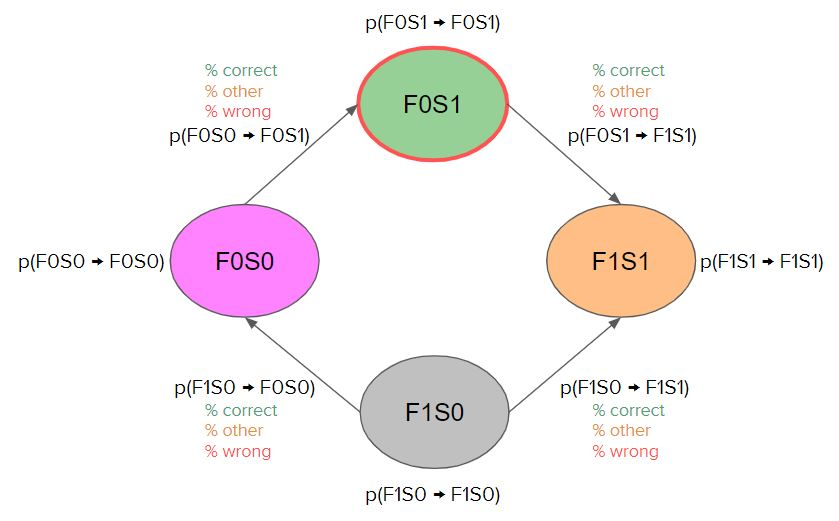
\includegraphics[width=.8\linewidth]{figures/fsm_example.jpg}
    \caption{ Example of a Finite State Machine }
    \label{fig:fsm_example}
\end{figure}
A few final notes on the FSM representation:
\begin{itemize}
    \item probabilities and percentages are extracted from the dev set
    \item self loop transitions are omitted from the graphical representation
    \item the sum of probababilities of outgoing transitions, including self loops, must be equal to 1
\end{itemize}

\subsubsection{Results on FIGER}
Only for these experiments, a reduced version of FIGER is used with the purpose to anticipate training convergence. The subset of the dataset is extracted by a random sample that counts approximately 267K training examples.
\paragraphn{Quantitative analysis 1 - Clause weights}
The performance in terms of \textit{macro f1 examples} obtained by varying the initial clause weights is available in Figure~\ref{fig:wandb_weights_comparison}. Looking at the graphs, we can observe a common behavior: regardless of the KB mode, the influence of different weights is visible only in the first 15-20 epochs (i.e., the red line in the graph is above the others in the initial epochs). Especially for the Hybrid mode, we can see in Figure~\ref{fig:wandb_weights_comparison_h} how the largest weight gives a clear initial boost to the performance. However, the boost tends to diminish over the epochs until it disappears. Another interesting behavior can be found in Figure~\ref{fig:wandb_weights_avg_pred_start}, which shows the evolution of the \textit{average predictions number} in the first 20 epochs. From the figures, we can observe that the larger the weight, the higher the number of predictions, and the larger the weight, the higher the performance. We can deduce from these results that the increased performance is due to an increased number of correct predictions, otherwise we would not see an increment in the performance. To conclude, we can say that a major influence of KENN helps the network to learn faster when it has not yet seen a big amount of training examples.
\\\\
\textit{\textbf{Note:} the previous considerations still apply to the other metrics not reported here}

\begin{figure}
     \centering
     \begin{subfigure}{0.8\textwidth}
         \centering
         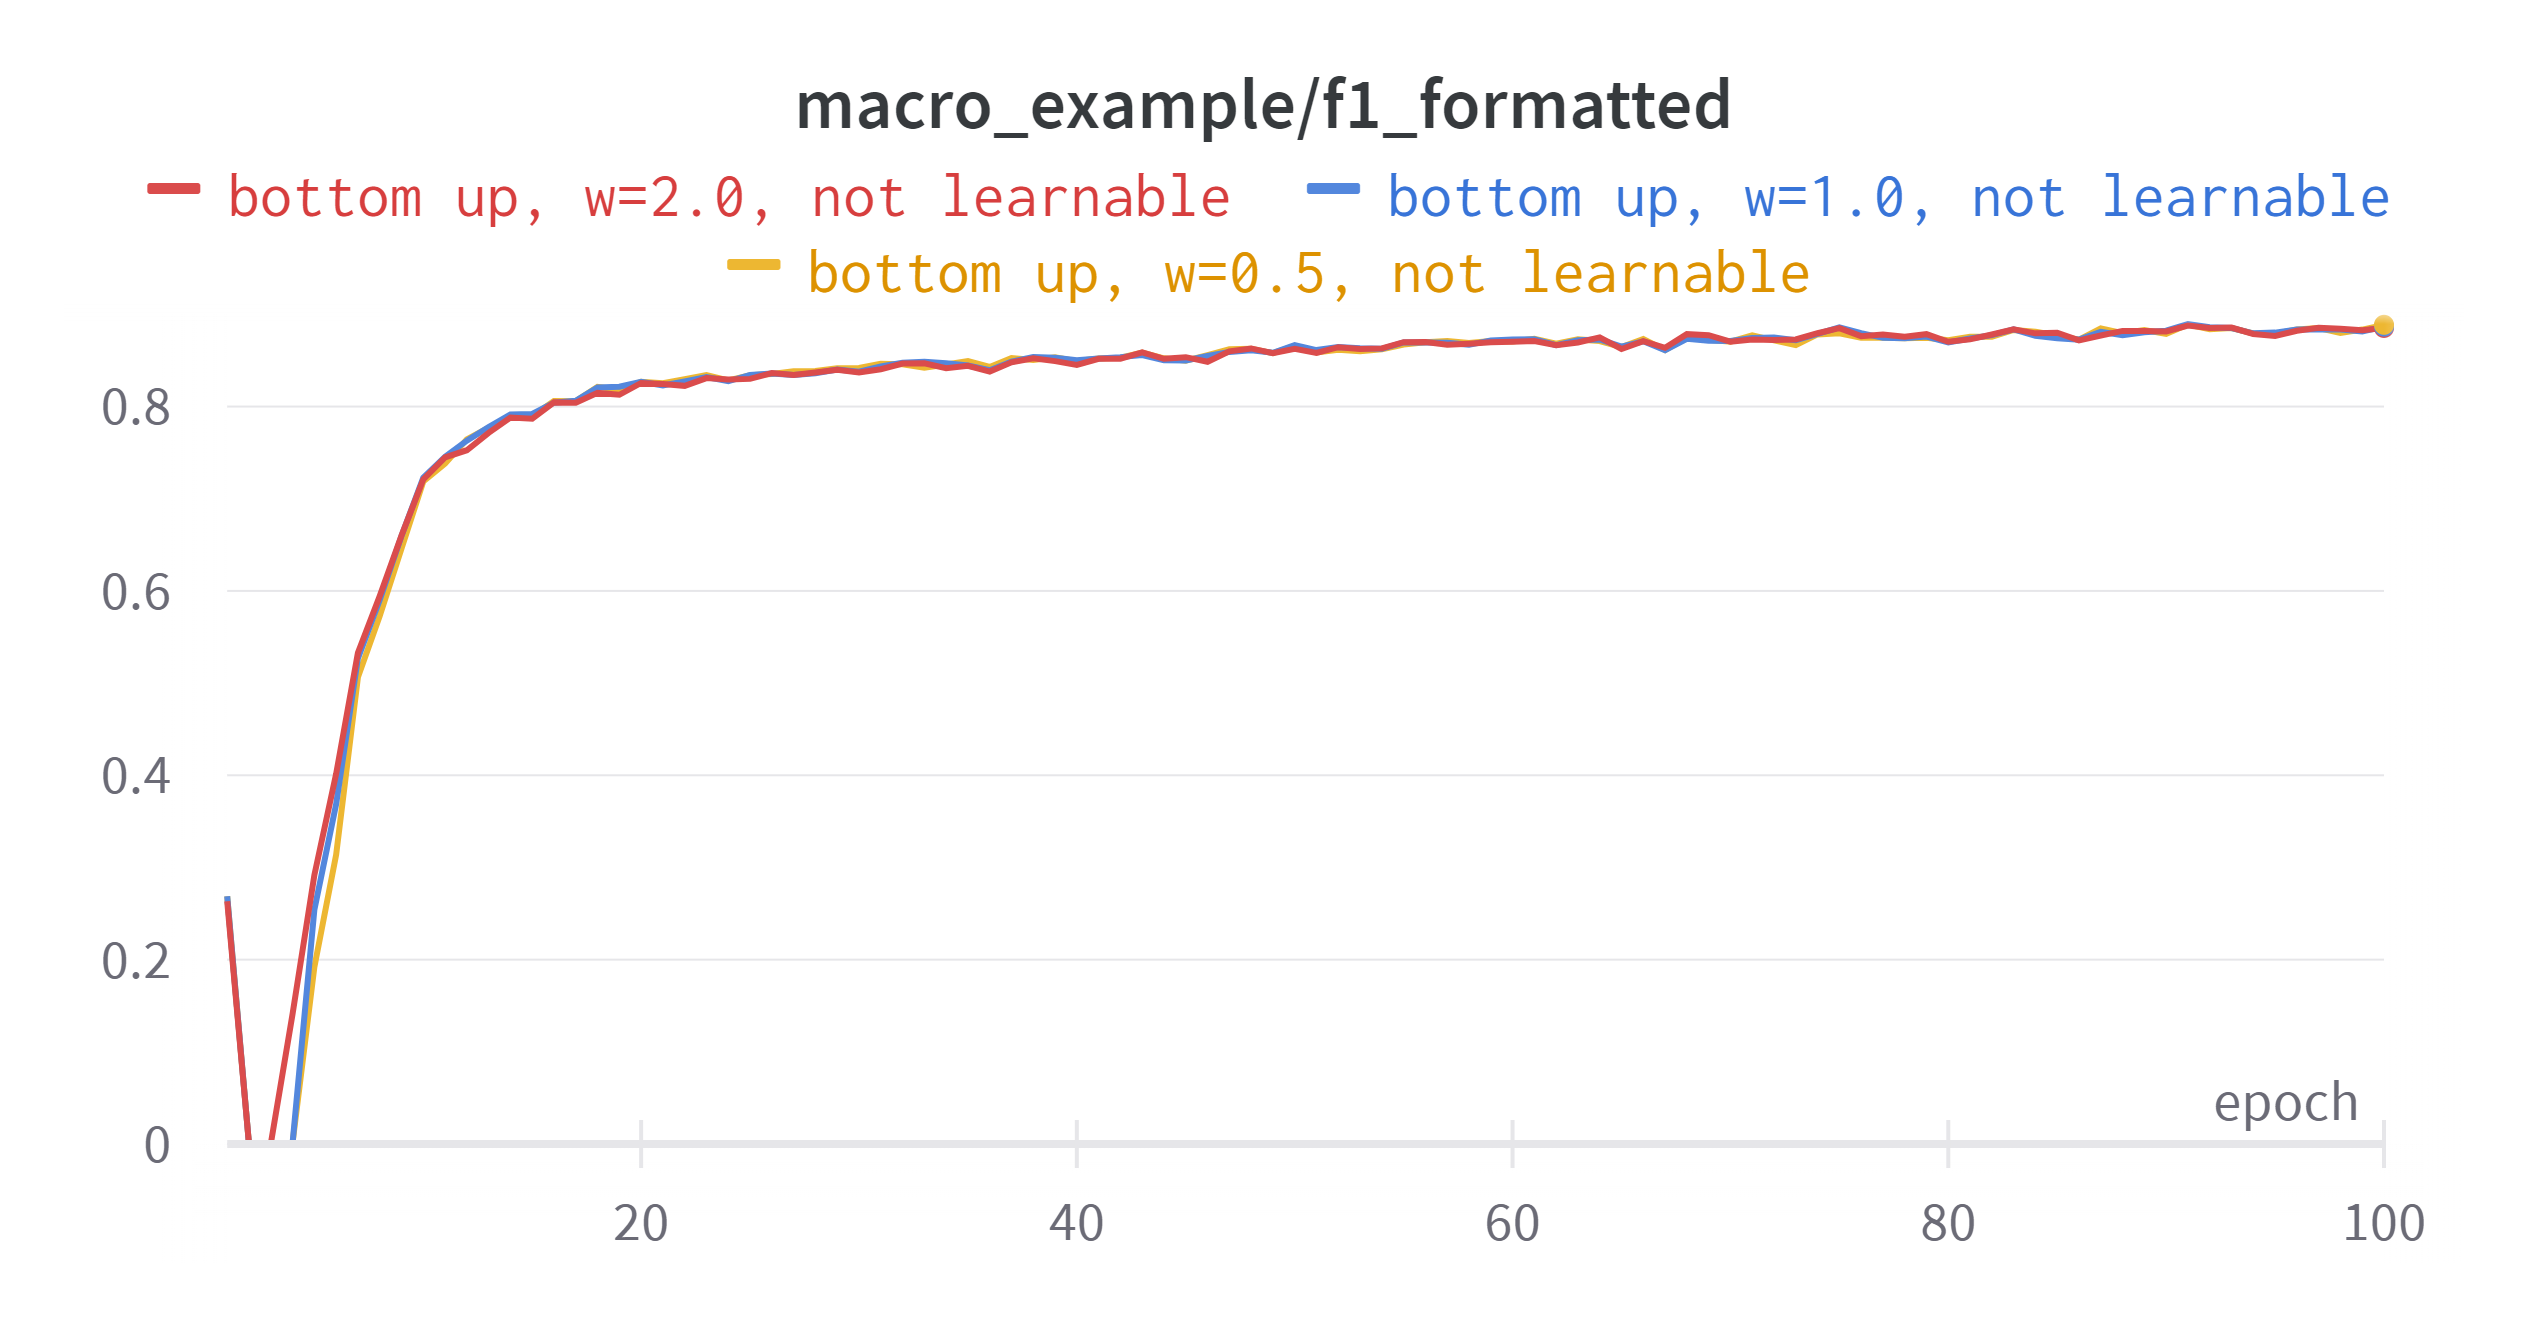
\includegraphics[width=\textwidth]{figures/wandb_weights_bottom_up_macro_ex_f1.png}
         \caption{Bottom Up}
     \end{subfigure}
     \vfill
     \begin{subfigure}{0.8\textwidth}
         \centering
         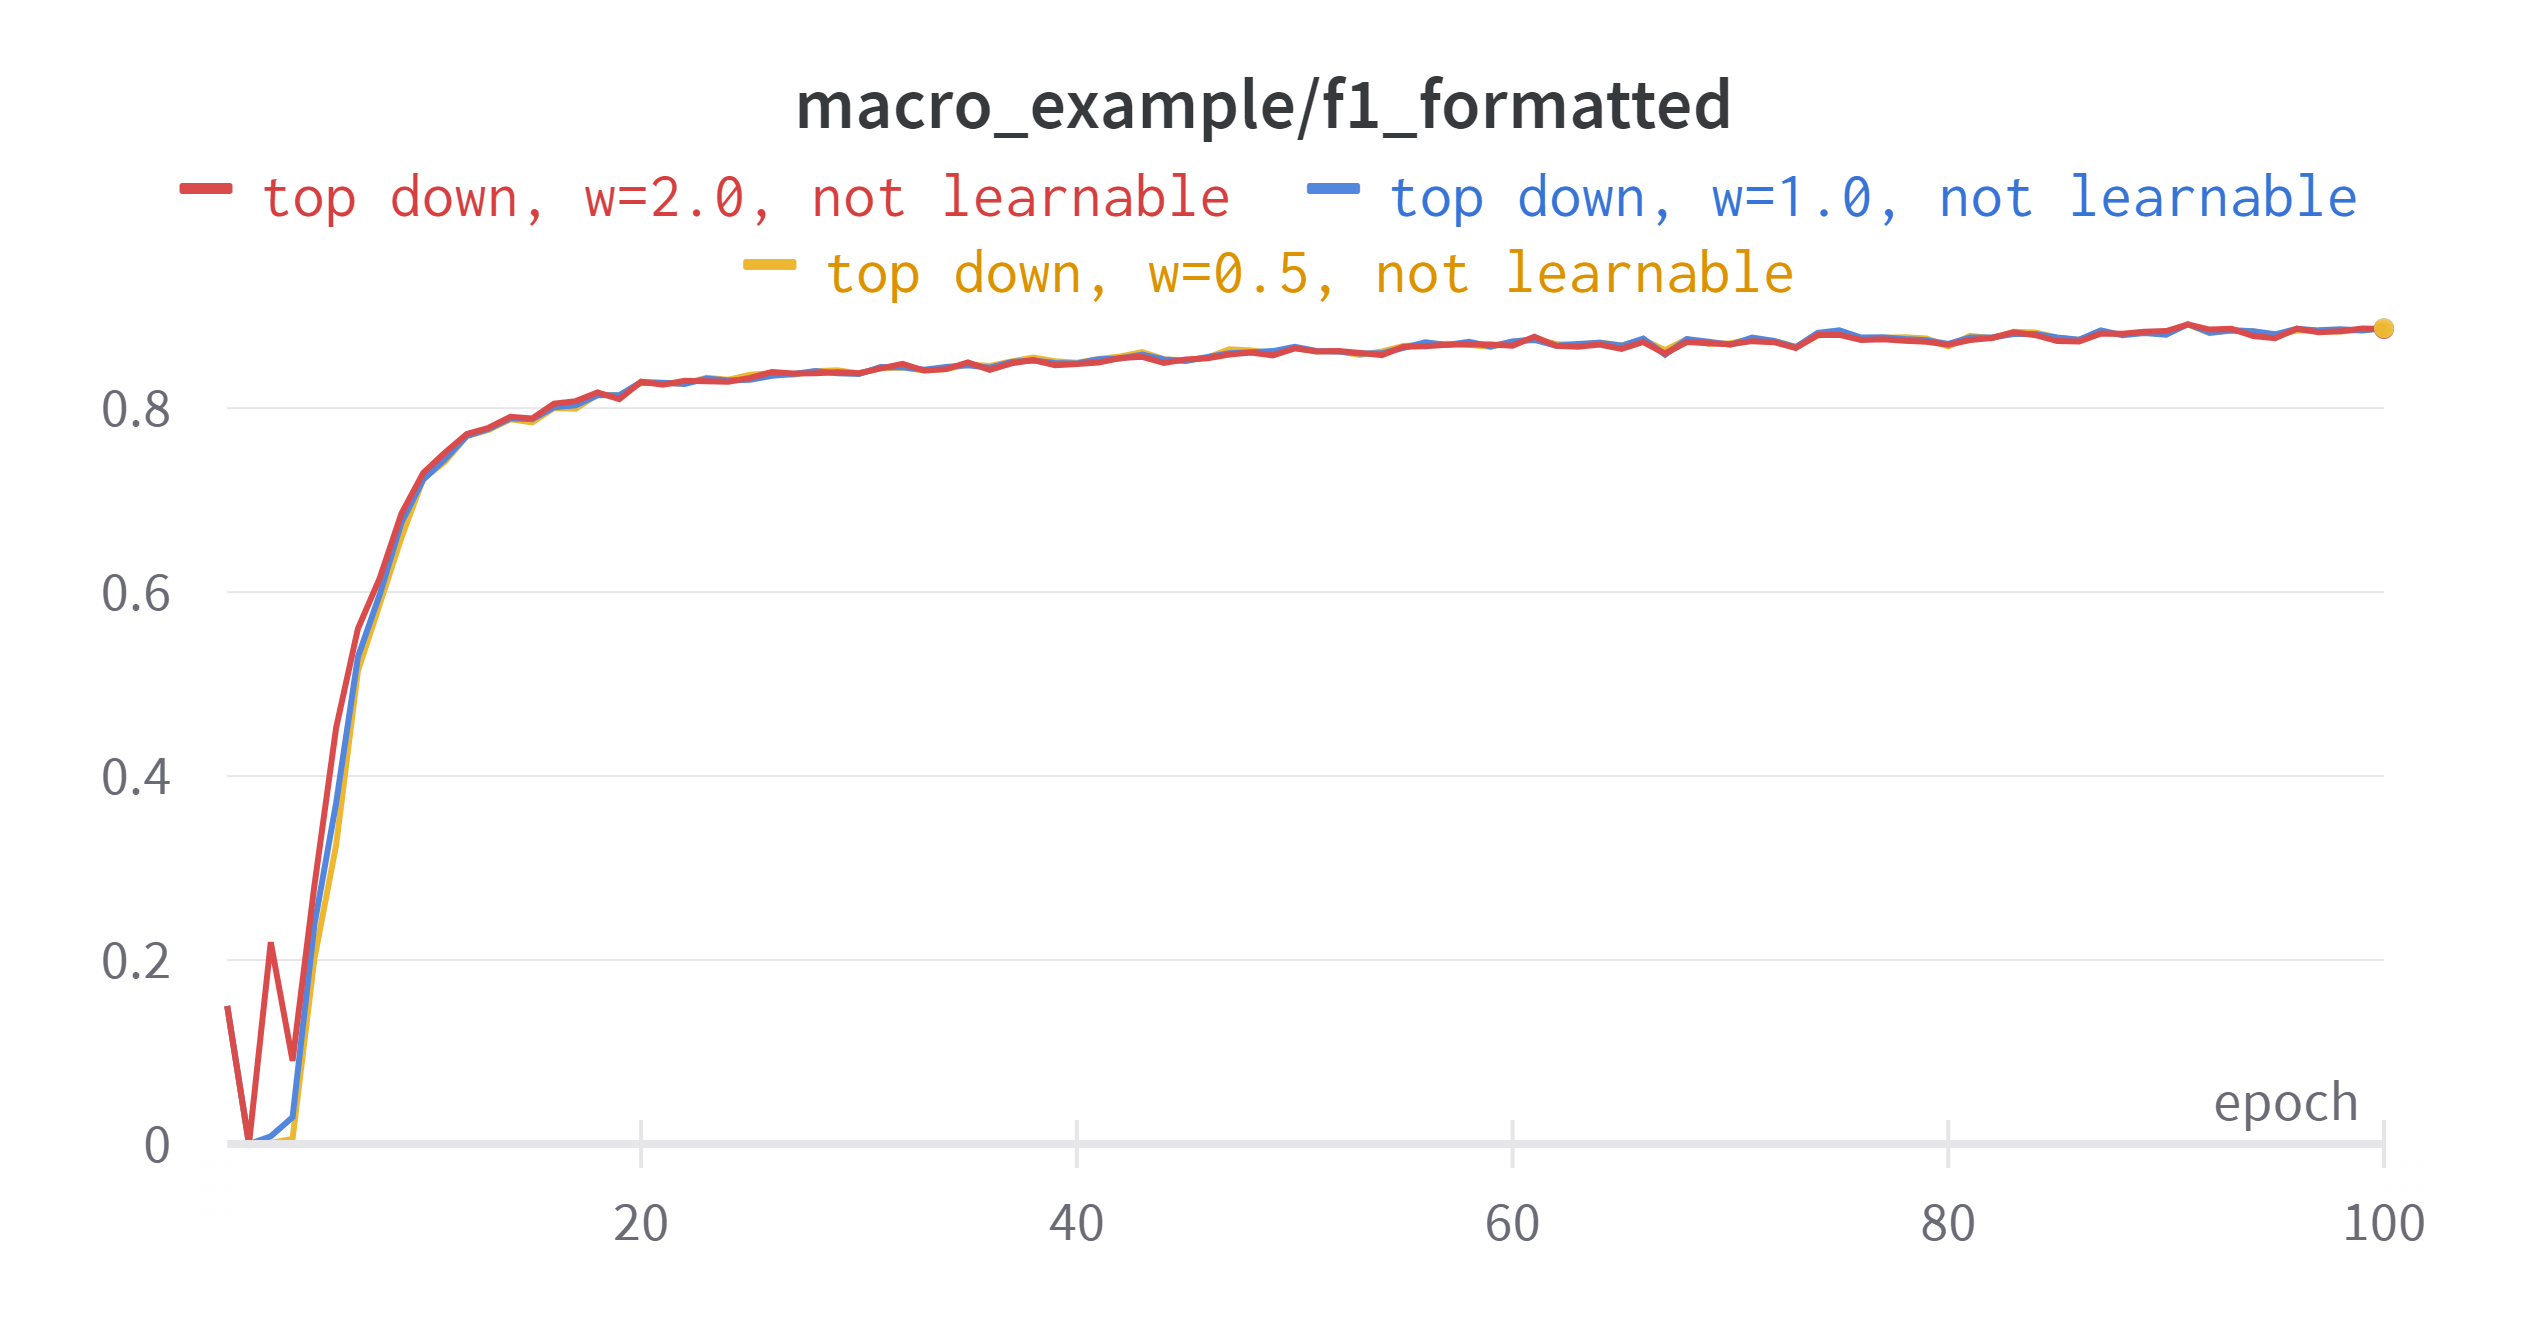
\includegraphics[width=\textwidth]{figures/wandb_weights_top_down_macro_ex_f1.png}
         \caption{Top Down}
     \end{subfigure}
     \vfill
     \begin{subfigure}{0.8\textwidth}
         \centering
         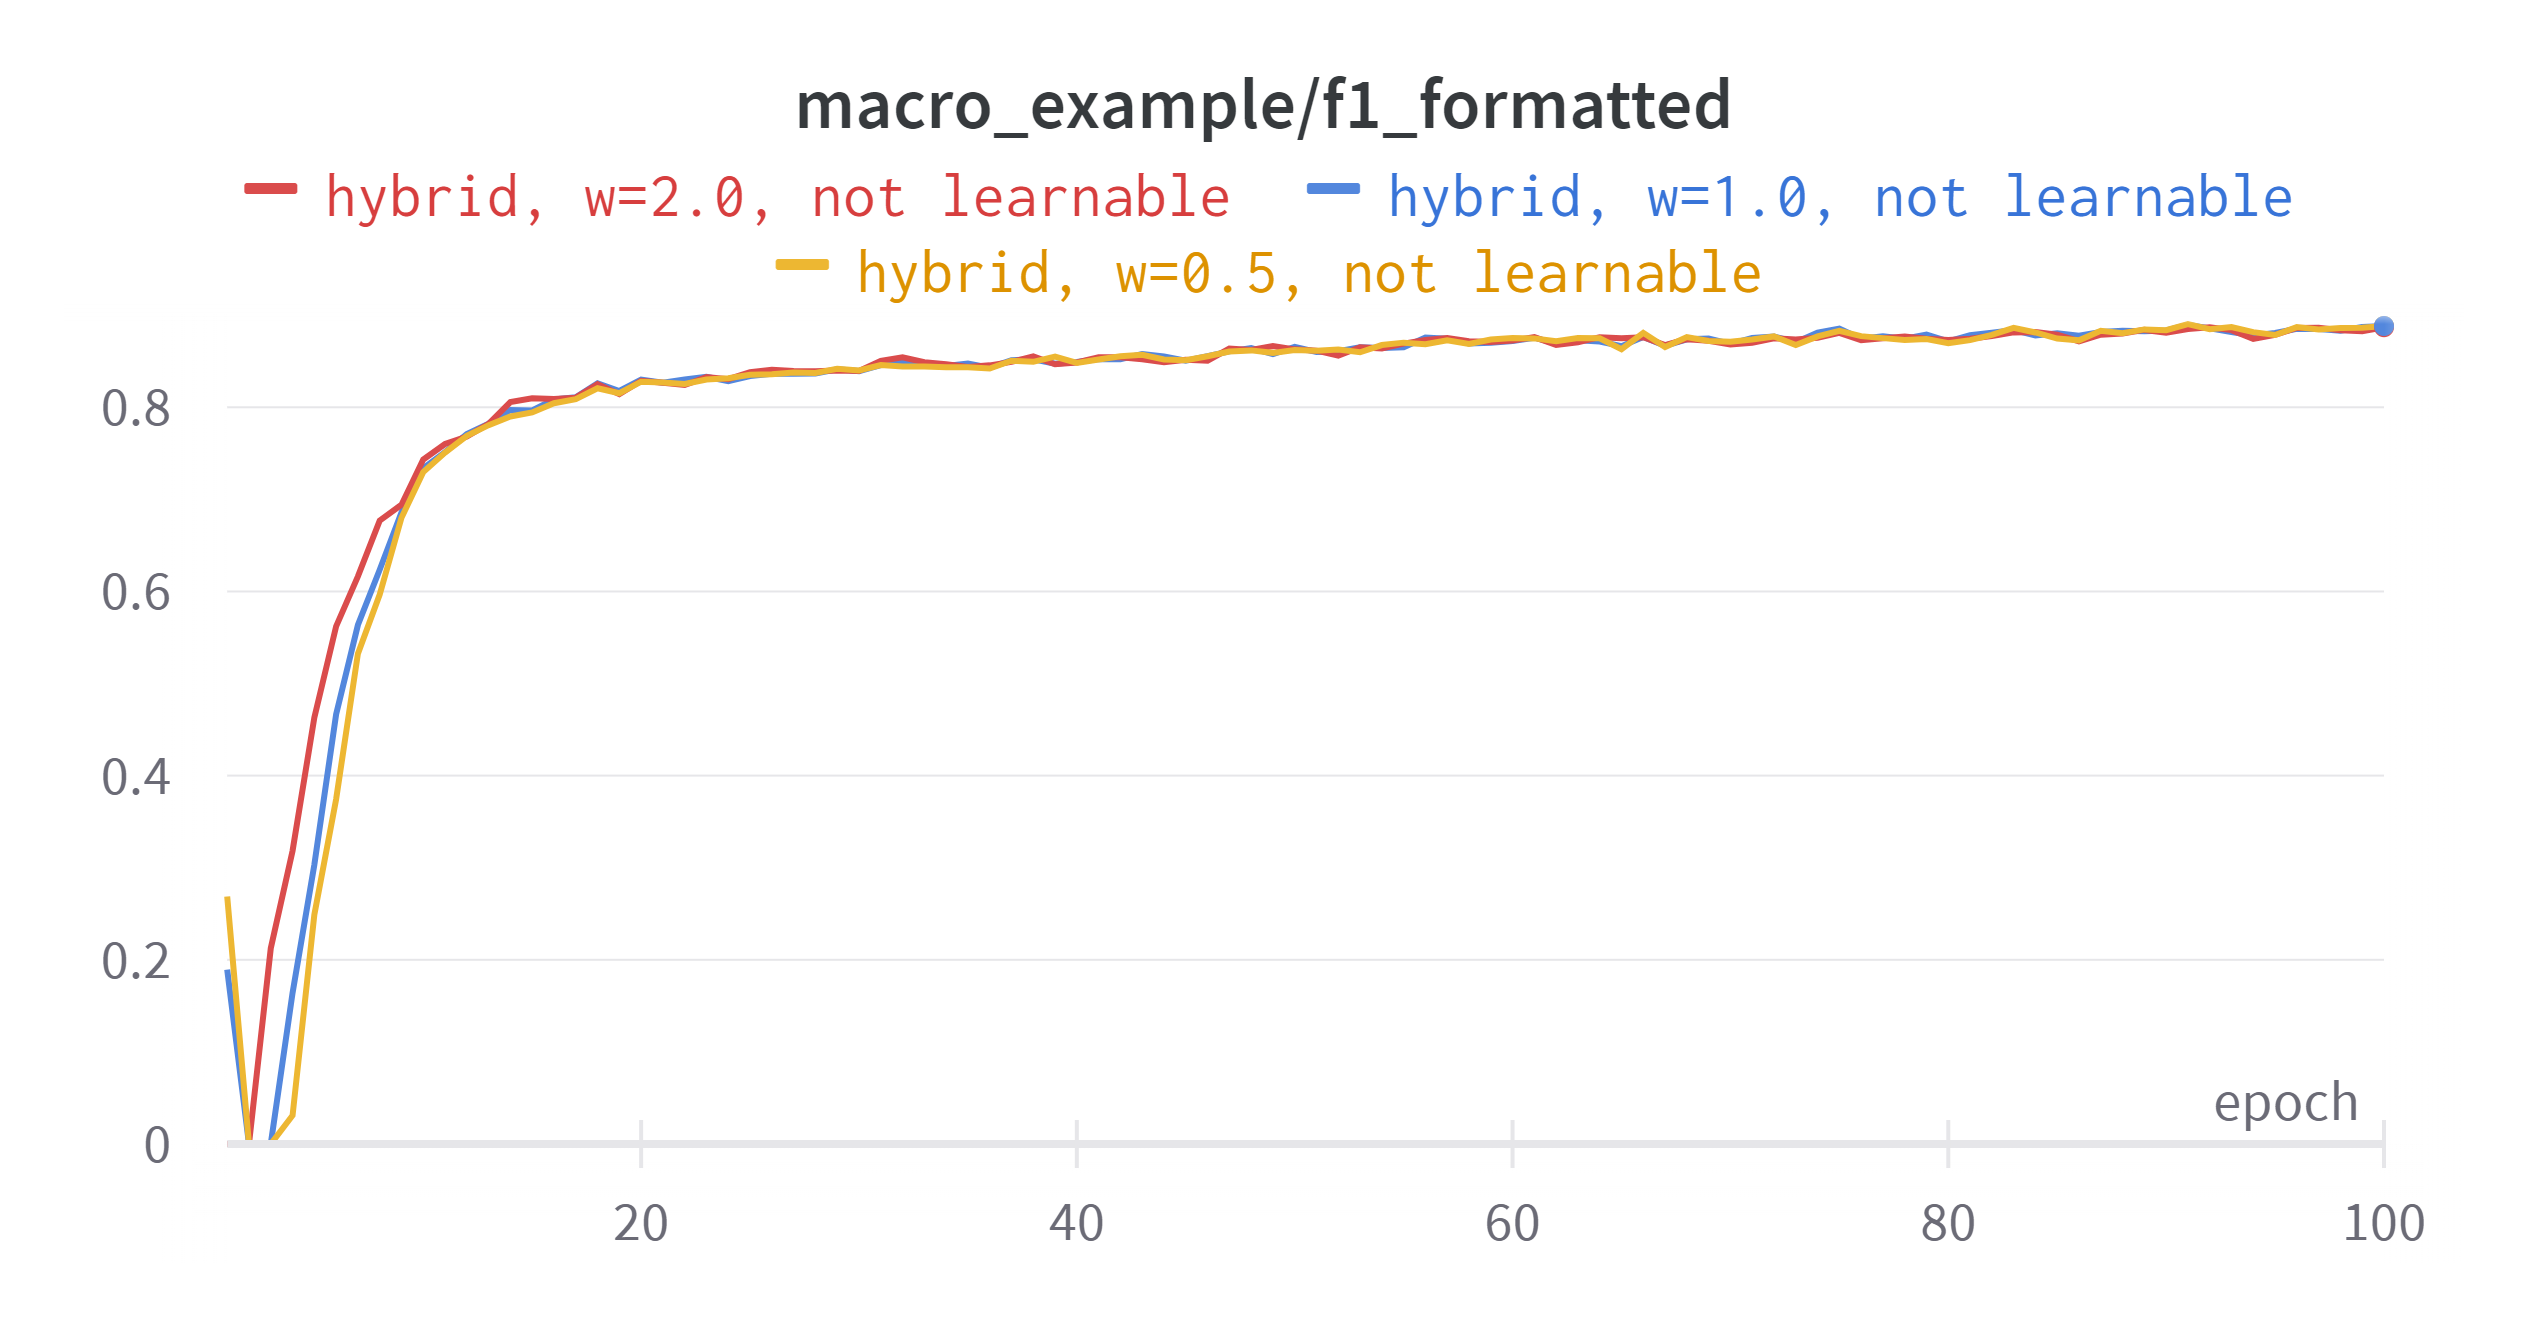
\includegraphics[width=\textwidth]{figures/wandb_weights_hybrid_macro_ex_f1.png}
         \caption{Hybrid}
         \label{fig:wandb_weights_comparison_h}
    \end{subfigure}
        \caption{Comparison of \textit{macro f1 examples} by varying the clause weight for each KB mode, with DistilBERT-based models evaluated on the dev set of FIGER.}
        \label{fig:wandb_weights_comparison}
\end{figure}

\begin{figure}
     \centering
     \begin{subfigure}{0.8\textwidth}
         \centering
         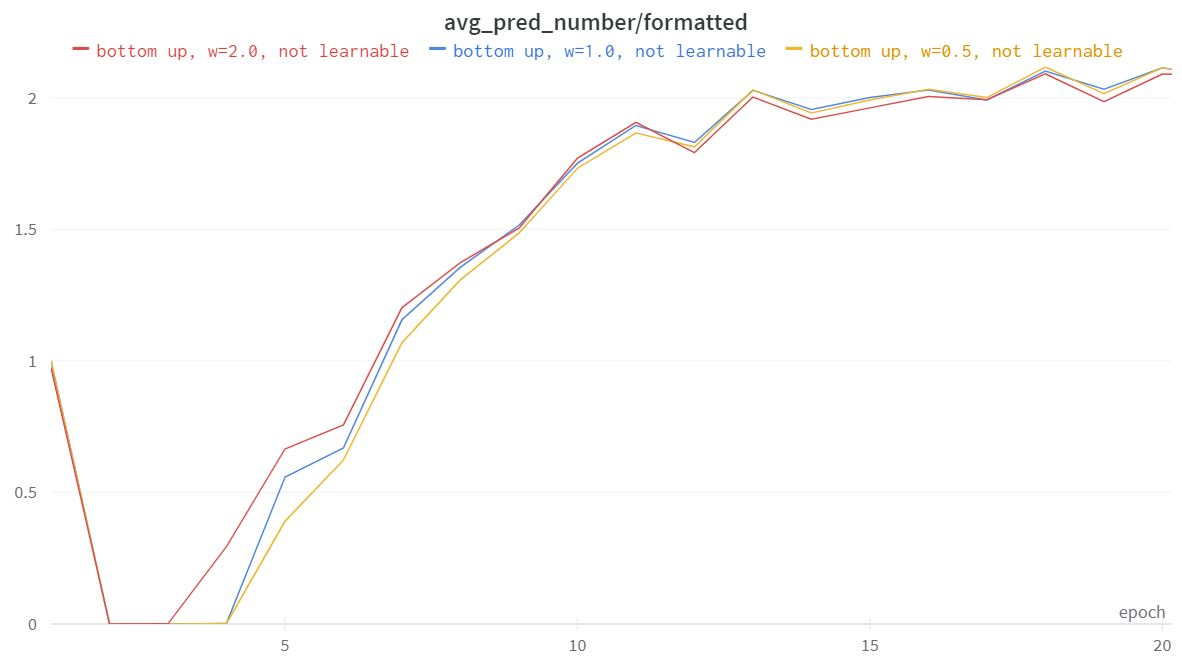
\includegraphics[width=\textwidth]{figures/wandb_weights_bottom_up_avg_pred_start.JPG}
         \caption{Bottom Up}
     \end{subfigure}
     \vfill
     \begin{subfigure}{0.8\textwidth}
         \centering
         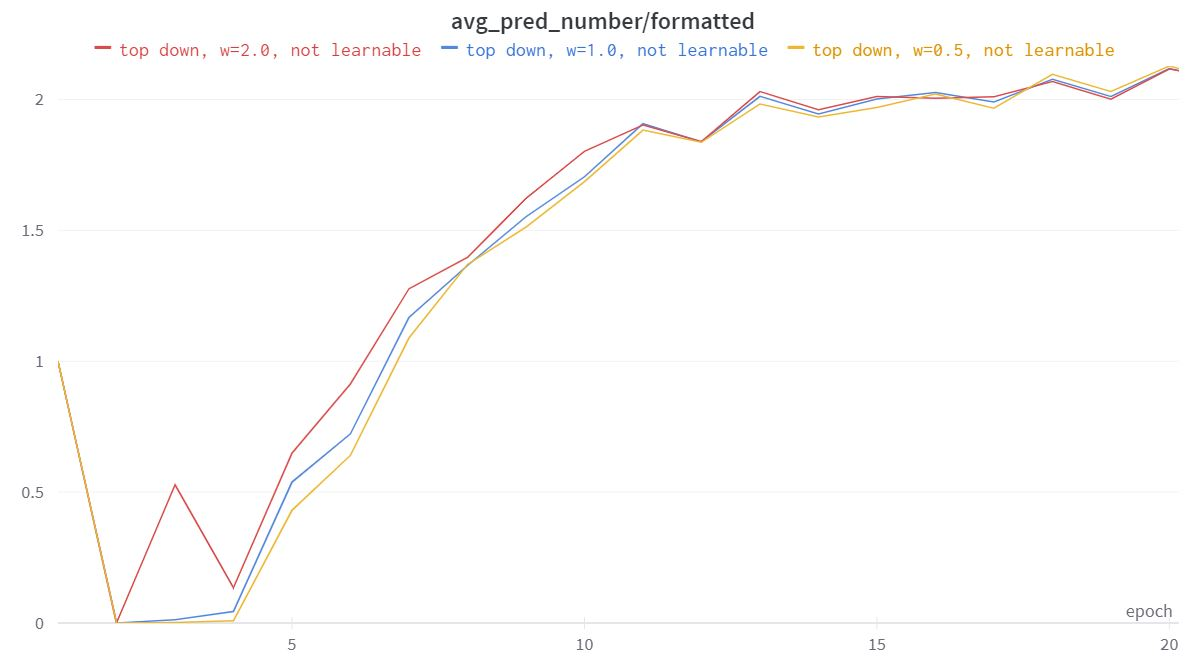
\includegraphics[width=\textwidth]{figures/wandb_weights_top_down_avg_pred_start.JPG}
         \caption{Top Down}
     \end{subfigure}
     \vfill
     \begin{subfigure}{0.8\textwidth}
         \centering
         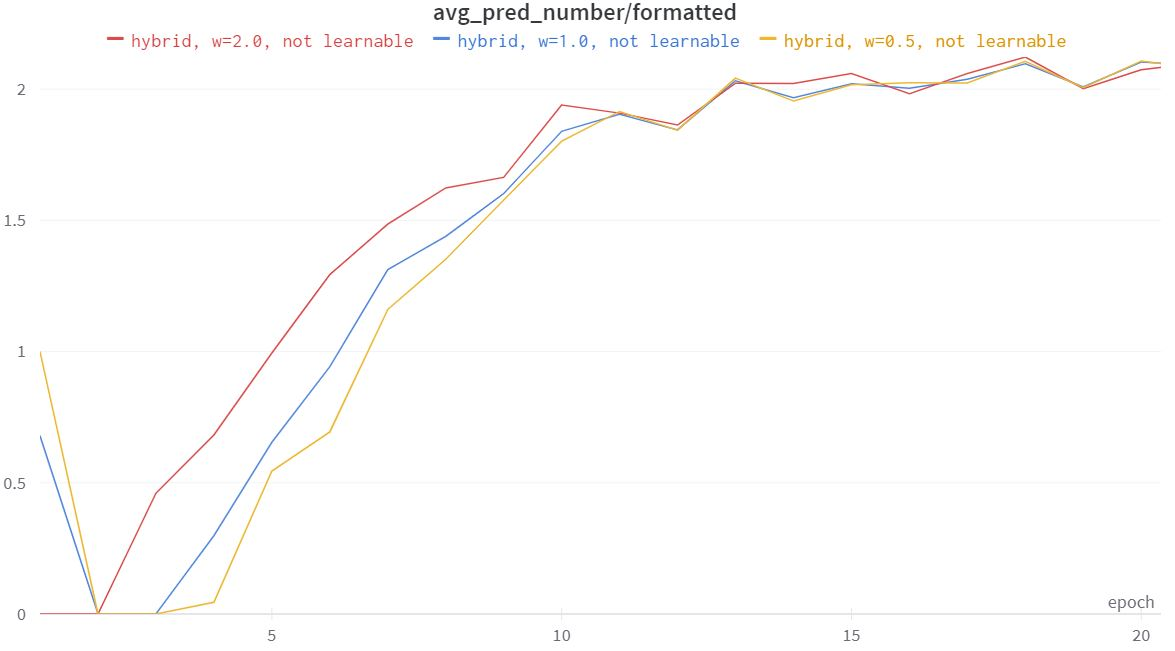
\includegraphics[width=\textwidth]{figures/wandb_weights_hybrid_avg_pred_start.JPG}
         \caption{Hybrid}
     \end{subfigure}
        \caption{Comparison of \textit{average predictions number} by varying the clause weight for each KB mode, with DistilBERT-based models evaluated on the dev set of FIGER. Zoom on the first 20 epochs.}
        \label{fig:wandb_weights_avg_pred_start}
\end{figure}

\paragraphn{Quantitative analysis 2 - KB modes}
Moving on to the comparison between the KB modes, 3 model instances per configuration were trained by varying the random seed. The initial clause weight is set to 2.0 because in the previous experiment was the one that obtained the biggest boost. Figure~\ref{fig:wandb_modes_comparison} reports the comparison graphs in terms of \textit{average predictions number}, \textit{macro f1 examples} and \textit{macro f1 classes }. Similarly to the comparison of the weight, we can draw some considerations about the first steps of the training. Starting from the \textit{average predictions number}, we can clearly observe that the baseline model (i.e, \textit{kb\_mode: - }) produces significantly fewer predictions than KENN in the early stage. In particular, we can notice that the baseline is not able to produce any prediction for the first 4 epochs. Since the pre-KENN network and the baseline network have the same initialization, the fact that KENN requires fewer epochs to make correct predictions is due to the use of logical knowledge.

\begin{figure}[h]
    \centering
    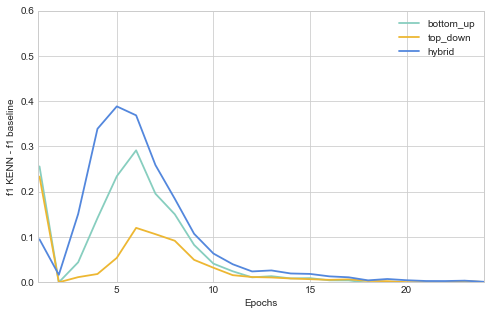
\includegraphics[scale=0.4]{figures/initial_boost.png}
    \caption{Difference between the \textit{macro f1 examples} scores of KENN and baseline models with DistilBERT encoder, evaluated on the dev set of FIGER. The curves are averaged over 3 random seeds. Zoom on the first 25 epochs.}
    \label{fig:initial_boost}
\end{figure}

The trend observed in the \textit{average predictions number} is also detectable by all the other metrics. Figure~\ref{fig:initial_boost} highlights the initial boost of KENN-based models by measuring the difference with respect to the baseline in terms of \textit{macro f1 examples}. The behavior that consolidates as the seeds vary is that Hybrid starts better than Bottom Up, which starts better than Top Down. The baseline model, instead, is the one with the slowest start. The cause of this initial ranking may be that the Hybrid mode can exploit the logical rules of both Bottom Up and Top Down modes. In the second part of the training, instead, the models converge to each other and keep improving together. The results of the final models are reported in Table~\ref{tab:kb_modes_comparison} and are very similar for each KB mode.
% Looking at the graphs in their entirety, there is not a dominant model. However, by looking at the \textit{macro f1 classes} graph we can observe that the baseline model is the only one which never takes the lead.
\begin{figure}
     \centering
     \begin{subfigure}{0.8\textwidth}
         \centering
         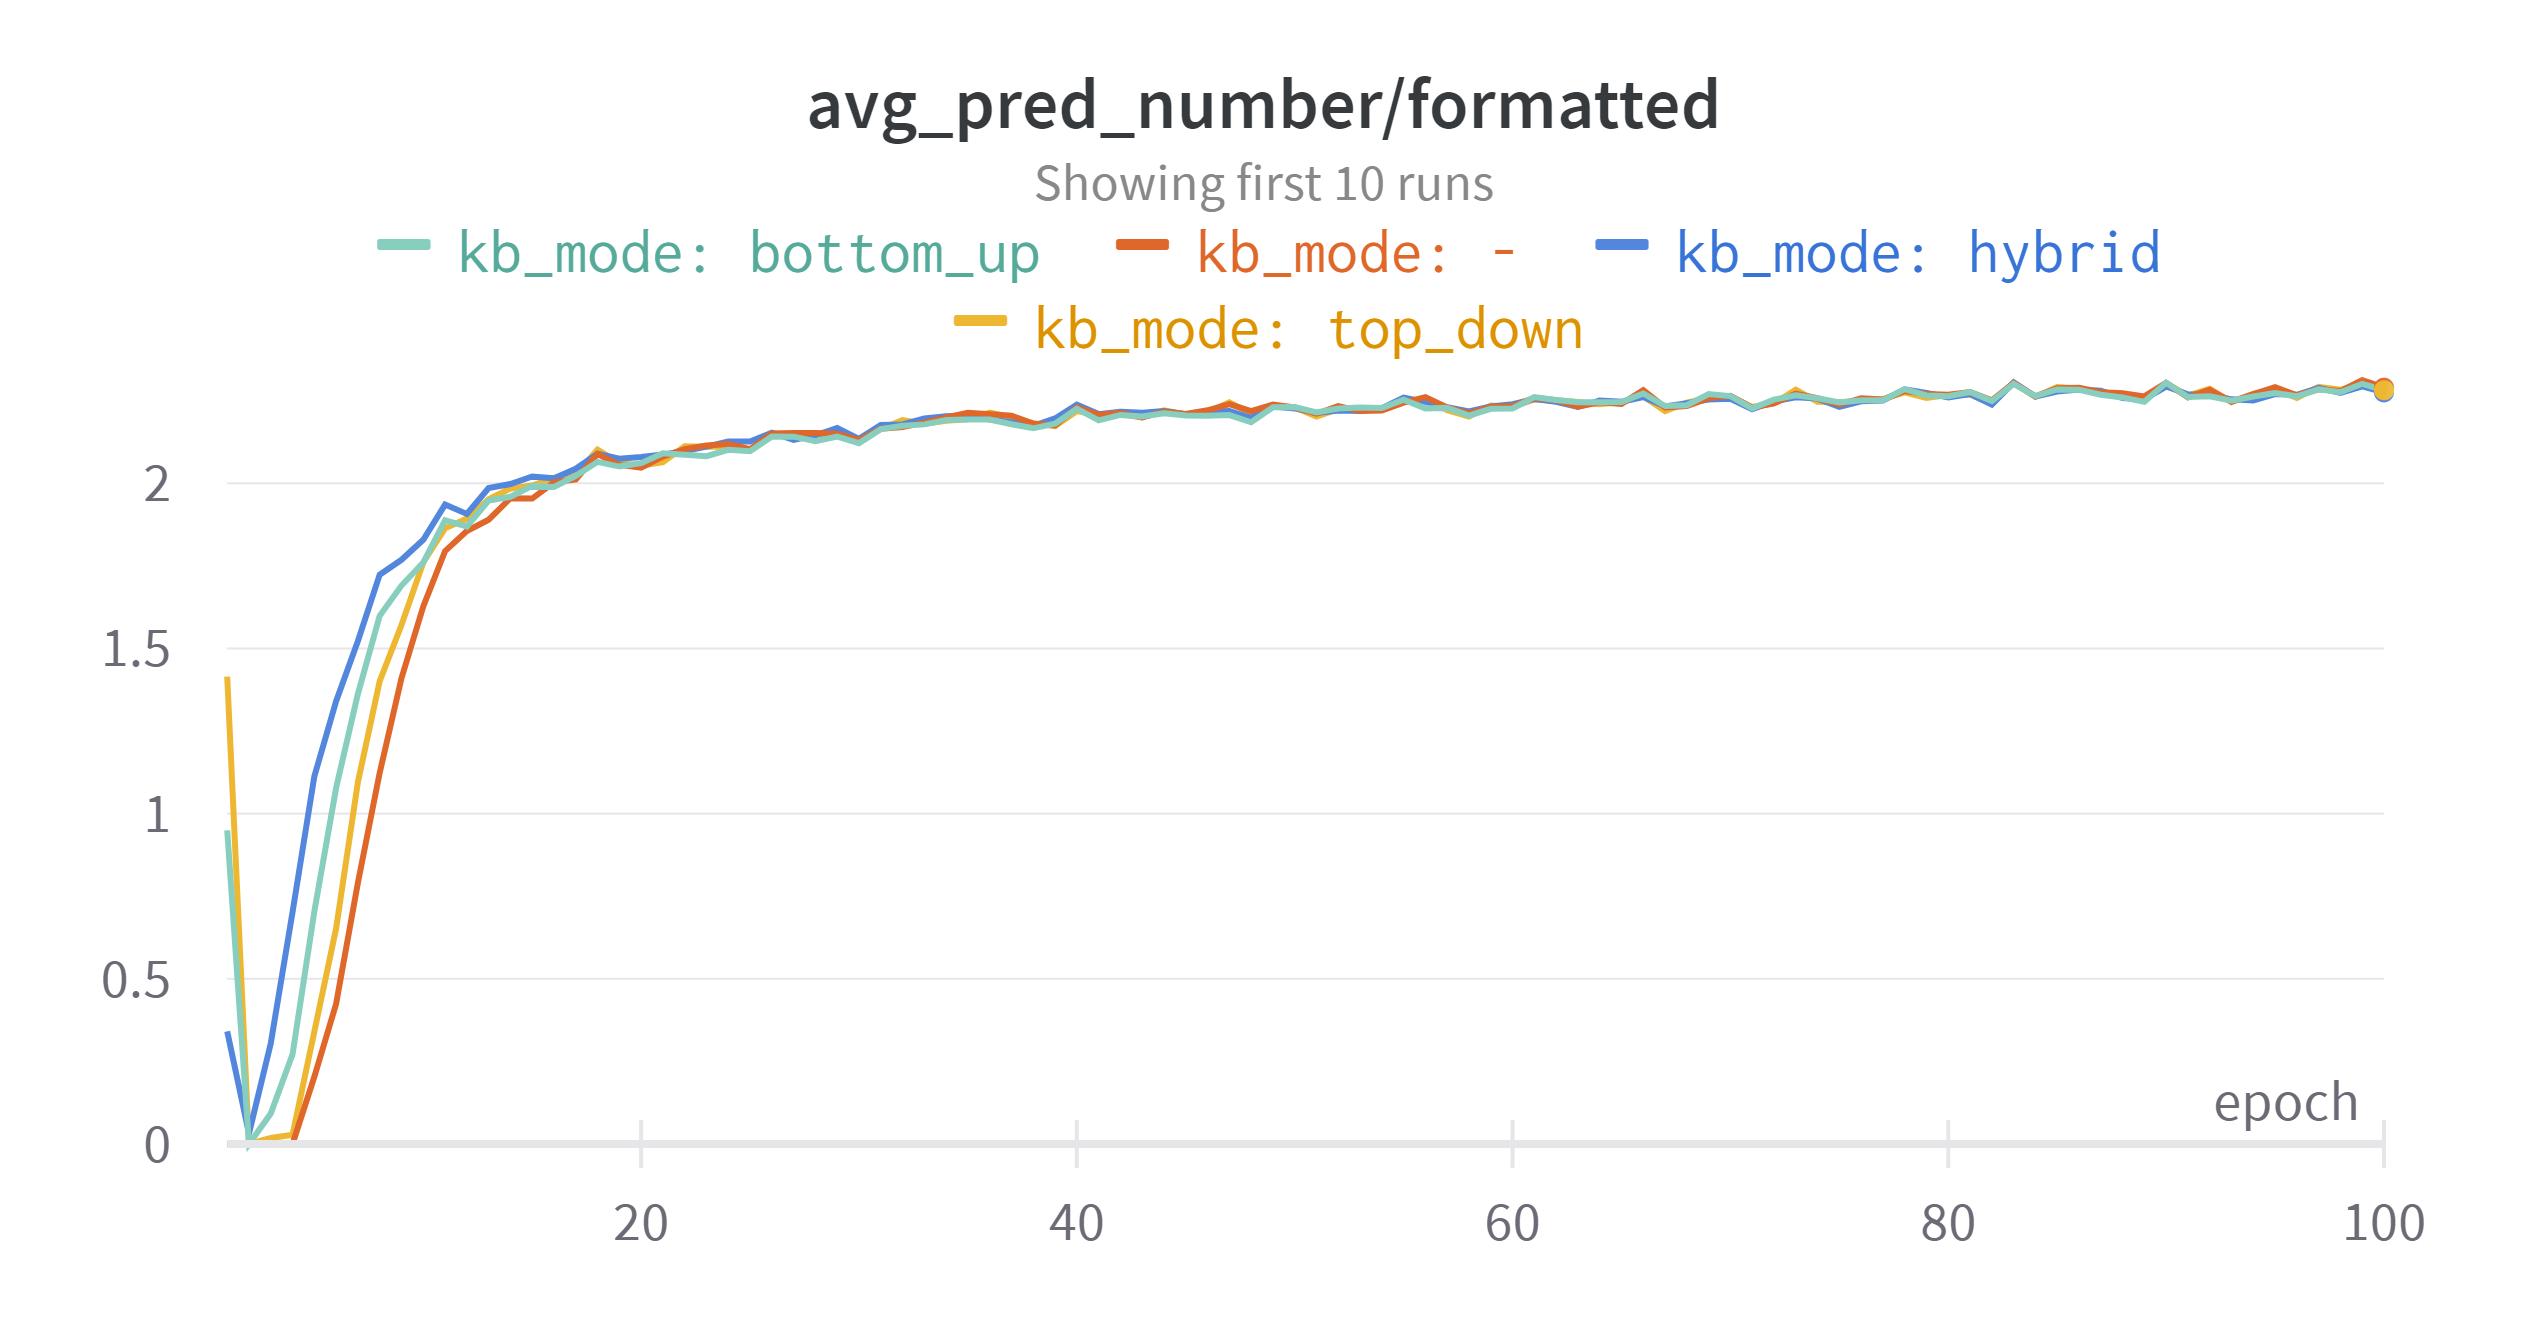
\includegraphics[width=\textwidth]{figures/wandb_modes_avg_pred.png}
         \caption{Average predictions number}
     \end{subfigure}
     \begin{subfigure}{0.8\textwidth}
         \centering
         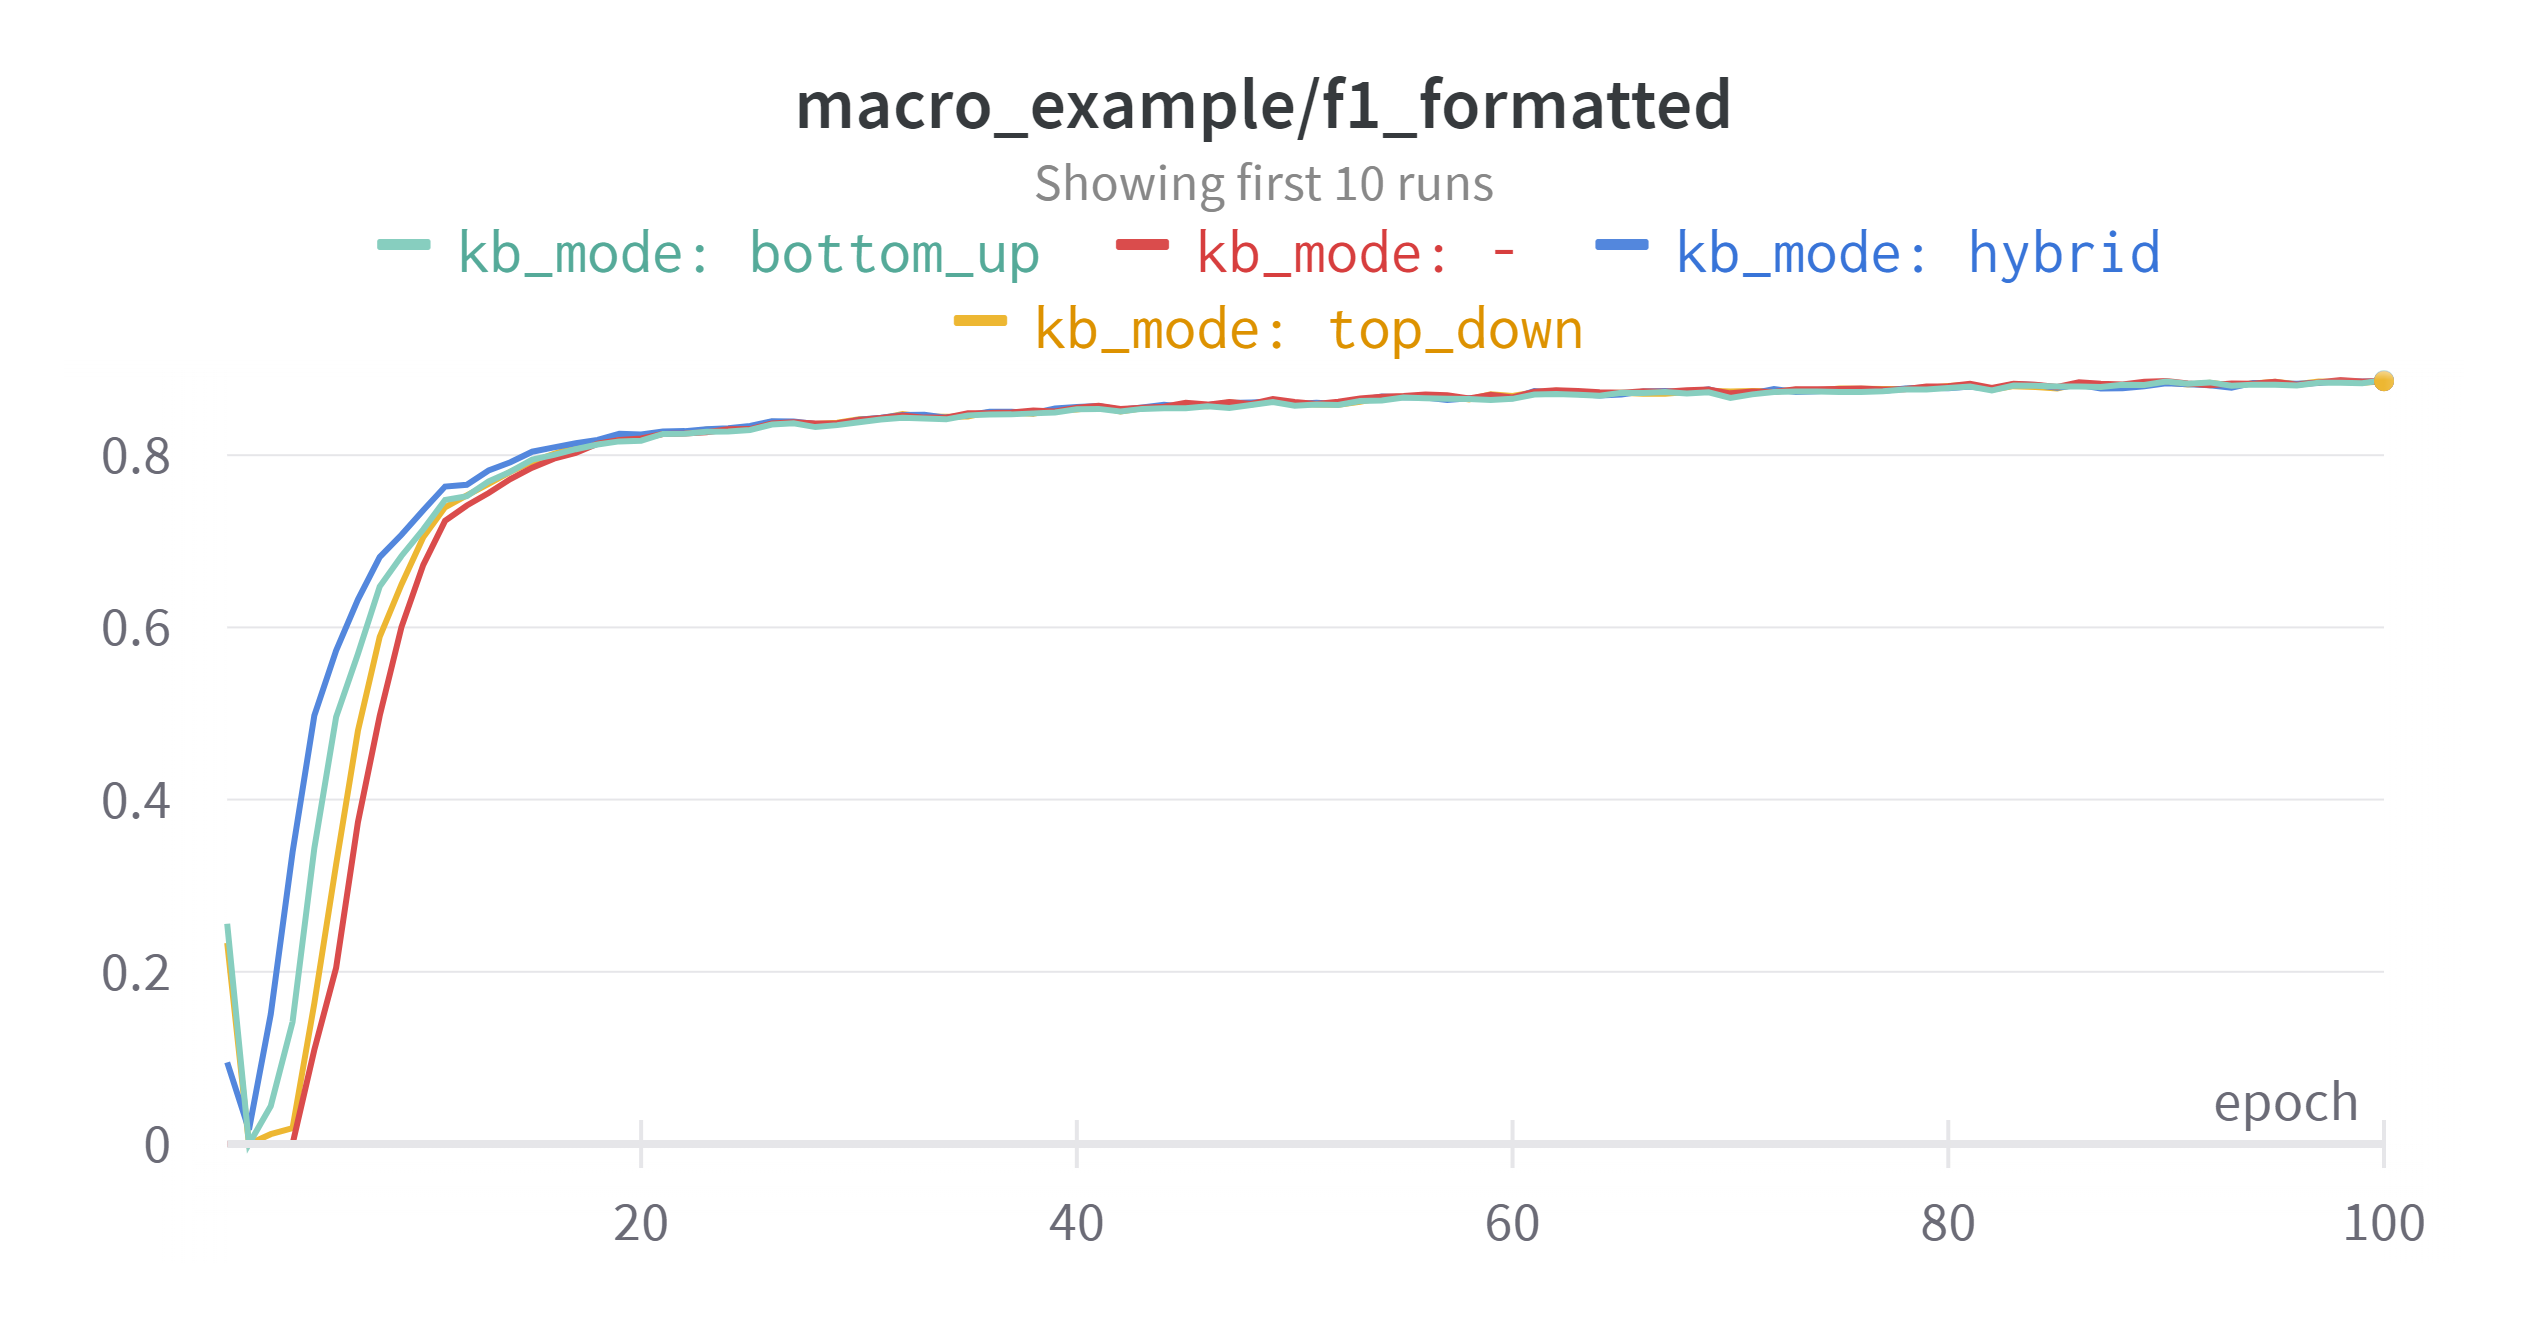
\includegraphics[width=\textwidth]{figures/wandb_modes_macro_ex_f1.png}
         \caption{Macro f1 examples}
     \end{subfigure}
     \begin{subfigure}{0.8\textwidth}
         \centering
         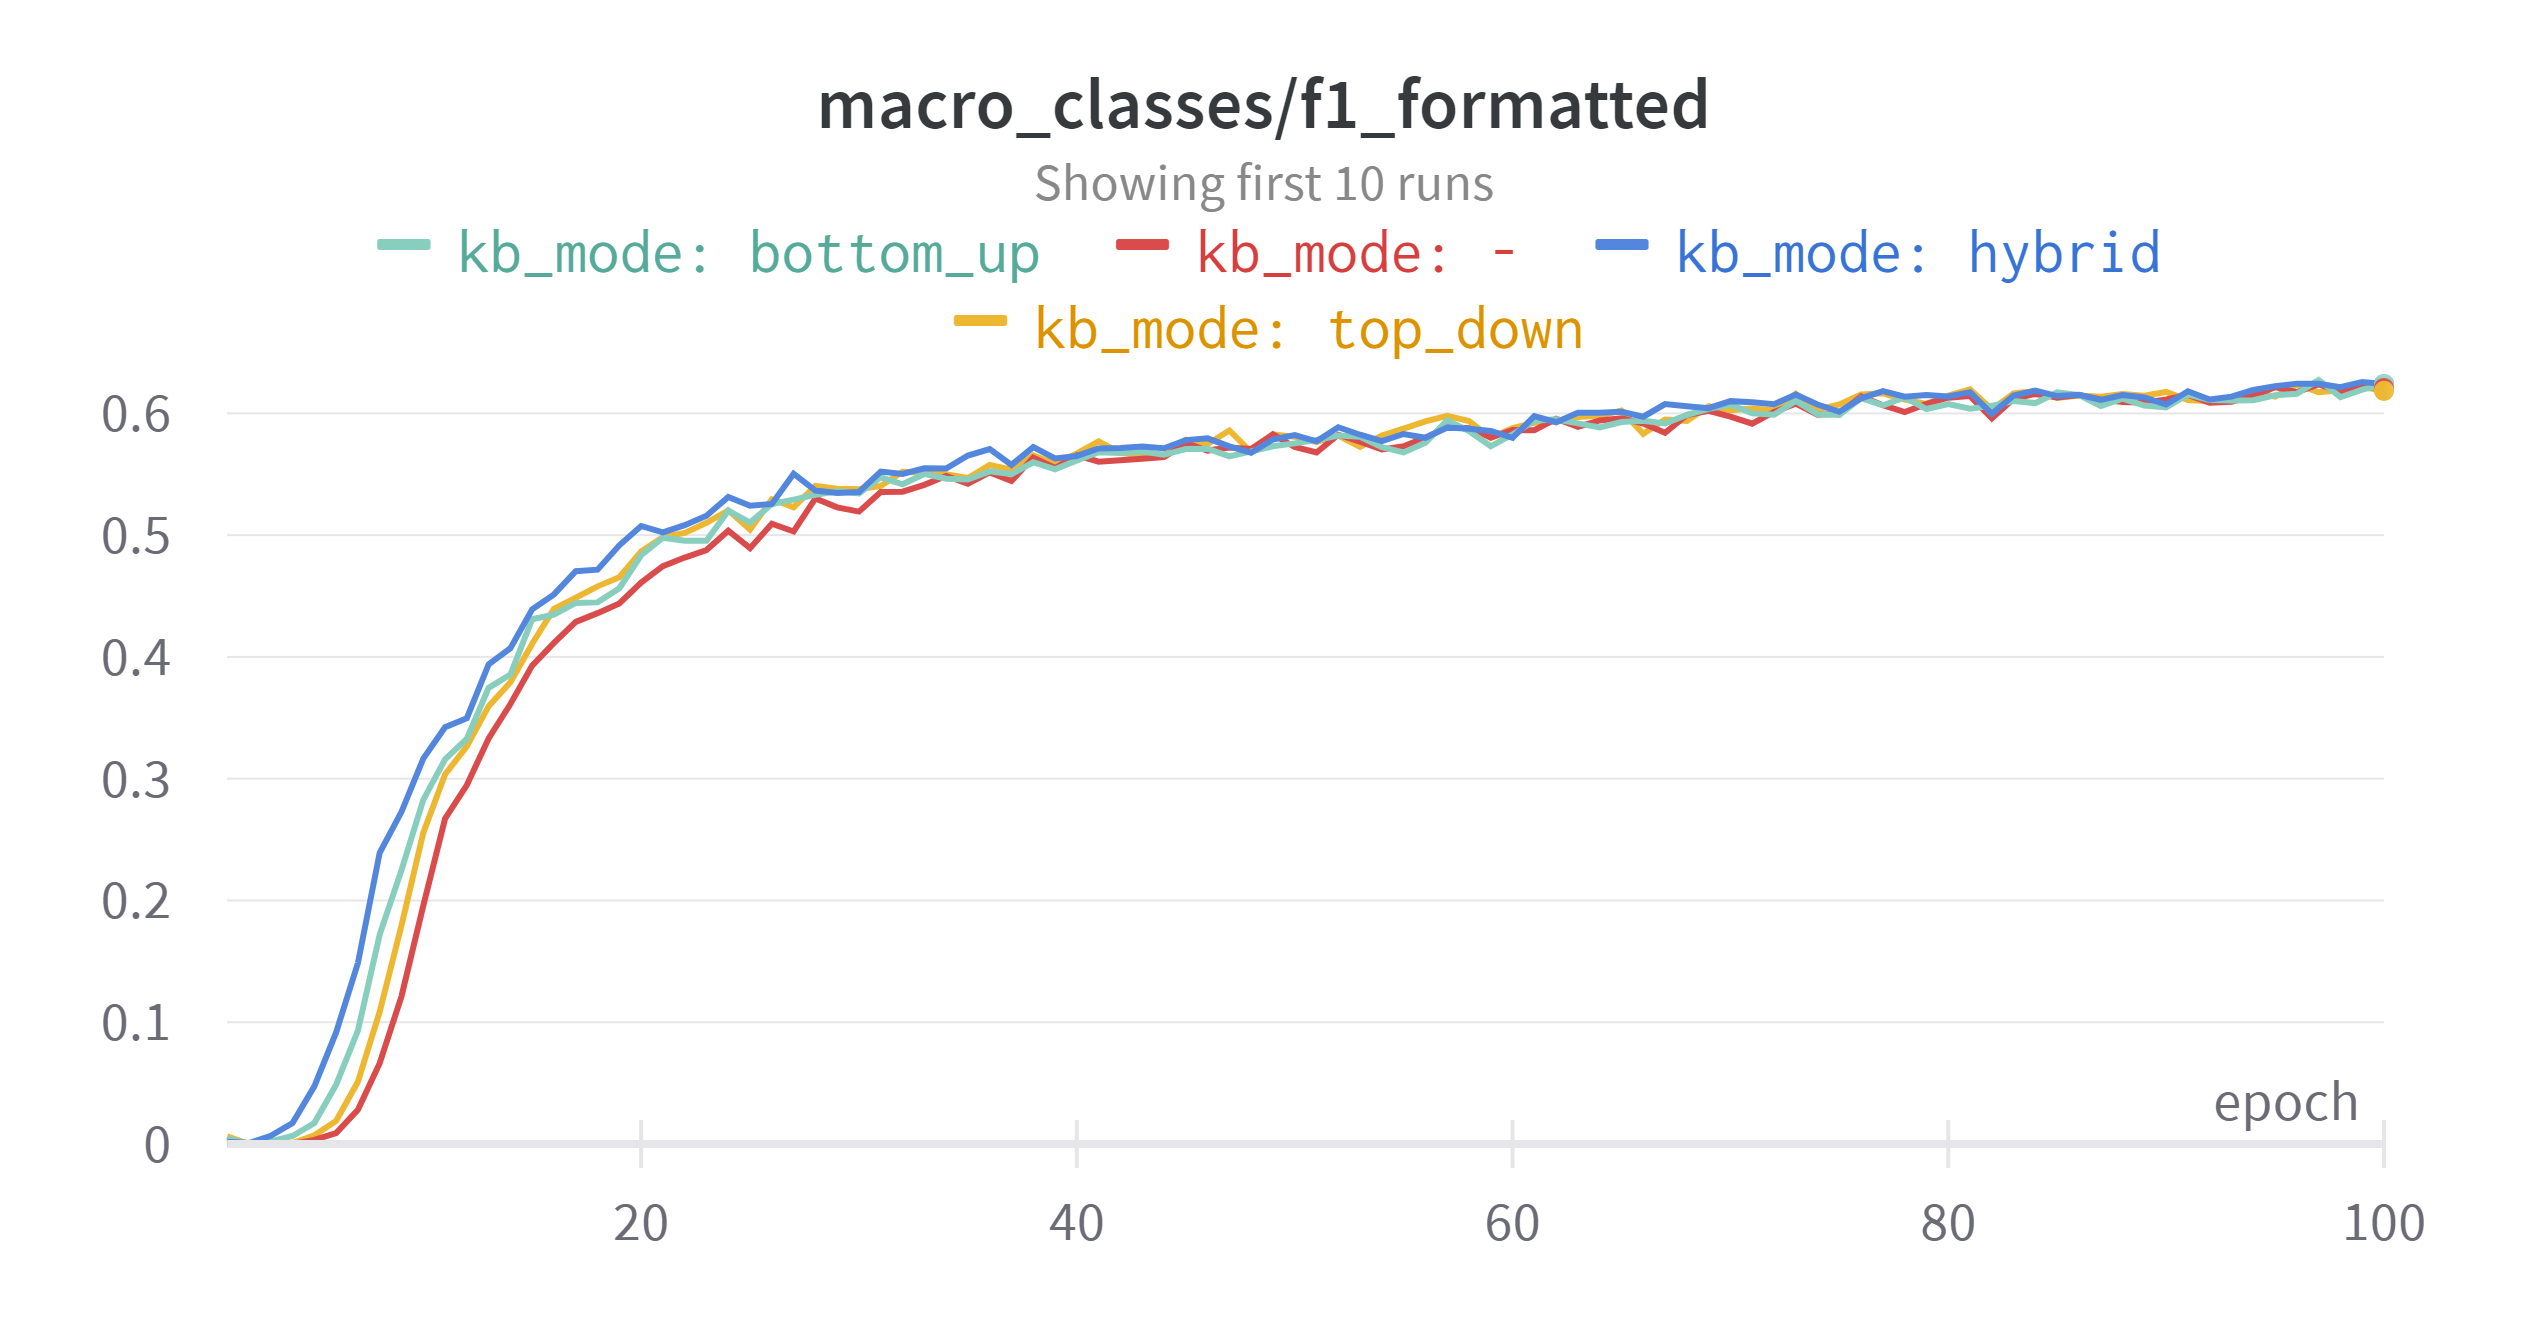
\includegraphics[width=\textwidth]{figures/wandb_modes_macro_class_f1.png}
         \caption{Macro f1 classes}
     \end{subfigure}
        \caption{Comparison between KENN with clause weights fixed to 2.0 and baseline model with DistilBERT encoder, evaluated on the dev set of FIGER. Zoom on the first 20 epochs.}
        \label{fig:wandb_modes_comparison}
\end{figure}

\begin{table}
\centering
\caption{Comparison between KENN with clause weights fixed to 2.0 and baseline model evaluated on the dev set of FIGER. Metrics at epoch 100 averaged over 3 seeds.}
\label{tab:kb_modes_comparison}
\resizebox{\columnwidth}{!}{\begin{tabular}{c|ccc|ccc|}
\cline{2-7}
\textbf{}                            & \multicolumn{3}{c|}{\textbf{Macro examples}}                                                                                                                                                                             & \multicolumn{3}{c|}{\textbf{Macro classes}}                                                                                                                                                                              \\ \hline
\multicolumn{1}{|c|}{\textbf{KB mode}} & \textbf{P}                                                             & \textbf{R}                                                             & \textbf{F1}                                                            & \textbf{P}                                                             & \textbf{R}                                                             & \textbf{F1}                                                            \\ \hline
\multicolumn{1}{|c|}{- (baseline)}       & \begin{tabular}[c]{@{}c@{}}0.8944\\ $\pm$ 0.0009\end{tabular}          & \begin{tabular}[c]{@{}c@{}}0.8779\\ $\pm$ 0.0033\end{tabular}          & \begin{tabular}[c]{@{}c@{}}0.8861\\ $\pm$ 0.0021\end{tabular}          & \begin{tabular}[c]{@{}c@{}}0.6499\\ $\pm$ 0.0152\end{tabular}          & \begin{tabular}[c]{@{}c@{}}0.5943\\ $\pm$ 0.0051\end{tabular}          & \begin{tabular}[c]{@{}c@{}}0.6208\\ $\pm$ 0.0091\end{tabular}          \\ \hline
\multicolumn{1}{|c|}{Bottom Up}      & \begin{tabular}[c]{@{}c@{}}0.8963\\ $\pm$ 0.0.0020\end{tabular}        & \textbf{\begin{tabular}[c]{@{}c@{}}0.8783\\ $\pm$ 0.0047\end{tabular}} & \textbf{\begin{tabular}[c]{@{}c@{}}0.8872\\ $\pm$ 0.0020\end{tabular}} & \begin{tabular}[c]{@{}c@{}}0.6516\\ $\pm$ 0.0165\end{tabular}          & \textbf{\begin{tabular}[c]{@{}c@{}}0.5986\\ $\pm$ 0.0110\end{tabular}} & \begin{tabular}[c]{@{}c@{}}0.6239\\ $\pm$ 0.0115\end{tabular}          \\ \hline
\multicolumn{1}{|c|}{Top Down}       & \begin{tabular}[c]{@{}c@{}}0.8944\\ $\pm$ 0.0008\end{tabular}          & \begin{tabular}[c]{@{}c@{}}0.8777\\ $\pm$ 0.0029\end{tabular}          & \begin{tabular}[c]{@{}c@{}}0.8860\\ $\pm$ 0.0013\end{tabular}          & \begin{tabular}[c]{@{}c@{}}0.6484\\ $\pm$ 0.0088\end{tabular}          & \begin{tabular}[c]{@{}c@{}}0.5913\\ $\pm$ 0.0112\end{tabular}          & \begin{tabular}[c]{@{}c@{}}0.6185\\ $\pm$ 0.0010\end{tabular}          \\ \hline
\multicolumn{1}{|c|}{Hybrid}         & \textbf{\begin{tabular}[c]{@{}c@{}}0.8965\\ $\pm$ 0.0028\end{tabular}} & \begin{tabular}[c]{@{}c@{}}0.8759\\ $\pm$ 0.0025\end{tabular}          & \begin{tabular}[c]{@{}c@{}}0.8861\\ $\pm$ 0.0017\end{tabular}          & \textbf{\begin{tabular}[c]{@{}c@{}}0.6533\\ $\pm$ 0.0185\end{tabular}} & \begin{tabular}[c]{@{}c@{}}0.5974\\ $\pm$ 0.0050\end{tabular}          & \textbf{\begin{tabular}[c]{@{}c@{}}0.6241\\ $\pm$ 0.0112\end{tabular}} \\ \hline
\end{tabular}}
\end{table}

\paragraphn{Quantitative analysis 3 - Metrics per type}
We can observe some interesting behaviors by computing the metrics grouped per types F and S. Focusing on epoch 4 (i.e., the last epoch before the baseline model starts making predictions), it emerges that KENN predicts only types F. This result makes sense since an F type should be easier to predict than an S type, which is more specific. More in detail, Bottom Up and Top Down modes can lead the model to make predictions exclusively on the type \texttt{/location}, reaching an f1 score of 0.595 and 0.441 respectively. The Hybrid model, which achieves an f1 score of 0.747 on \texttt{/location}, can also predict instances of type \texttt{/person} and \texttt{/organization}.

If we now focus on epoch 100, we can observe that Bottom Up performs better than Top Down on types F, with an f1 score of 0.661 and 0.646 respectively. Conversely, if we group the metrics per type S, we can observe that Top Down is better than Bottom Up, with an f1 score of 0.563 and 0.546 respectively. This behavior is consistent with the nature of the different clauses: Bottom Up propagates the information to F, Top Down to S.

\paragraphn{Quantitative analysis - Conclusion}
This analysis points out that the more relevant differences are observable only at the beginning of the training. The initial gap between different clause weights is bridged after 15-20 epochs, as does the difference between the KB modes. The same behavior can be observed when comparing KENN to the baseline model. The suspicion emerging from these considerations is that, at some point of the training, the baseline model becomes as powerful as the KENN-based models. 
%This suspicion can also be extended to the pre-KENN network, which increases its prediction capabilities epoch after epoch, needing less and less KENN's help.
From this premises we can sketch the following hypothesis: the pre-KENN network may adapt its output to obtain some desired predictions after the knowledge enhancement. This hypothesis will be further investigated with the analysis of the preactivations.
\paragraphn{Preactivations analysis 1 - Distributions}
We concluded the quantitative analysis leaving an open question: does the pre-KENN network adapt its predictions to KENN's action? To answer this question, we can start by examining the distribution of the preactivations of every final model. Each distribution will be split into two graphs to simplify the comparison by separating positive and negative predictions using different scales. Figure~\ref{fig:baseline_distrib} shows the distributions of the baseline model that will be used as a reference point. The values of $x$ are the preactivations of each type of each example, while the $y$ represents the frequency of a bin of preactivations.

We will start by comparing the positive predictions. In Figure~\ref{fig:kenn_pos_distrib} we can find the positive distributions of the KENN-based models. The first thing we can observe is that each KB mode produces very different pre-KENN distributions. If we look at the means (Bottom Up: 2.706, Top Down: 3.633, Hybrid: 2.227) and standard deviations (Bottom Up: 1.737, Top Down: 2.190, Hybrid: 1.434), we can also assert that they differ a lot from the baseline positive distribution (mean: 4.246, standard deviation: 2.228). On the contrary, the situation is completely different when looking at the post-KENN preactivations, since the intervention of KENN makes the distributions more similar to each other (means: 4.100$\pm$0.043, standard deviations: 2.058$\pm$0.038) and to the baseline. The same phenomenon can be observed by comparing the negative distribution of the baseline in Figure~\ref{fig:baseline_neg_distrib} to the pre-KENN and post-KENN negative distributions in Figure~\ref{fig:kenn_neg_distrib}.

\begin{figure}[H]
     \centering
     \begin{subfigure}{0.5\textwidth}
         \centering
         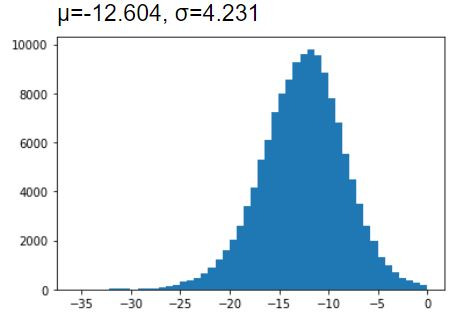
\includegraphics[width=\textwidth]{figures/baseline_neg.JPG}
         \caption{Negative preactivations}
         \label{fig:baseline_neg_distrib}
     \end{subfigure}
     \hfill
     \begin{subfigure}{0.475\textwidth}
         \centering
         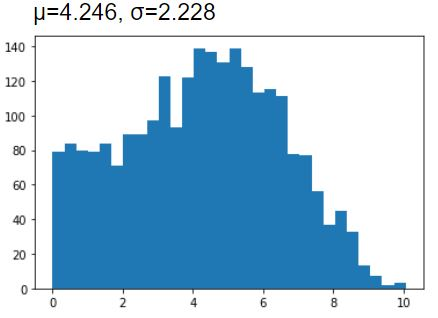
\includegraphics[width=\textwidth]{figures/baseline_pos.JPG}
         \caption{Positive preactivations}
         \label{fig:baseline_pos_distrib}
     \end{subfigure}
        \caption{Distribution of the baseline preactivations computed on the dev set of FIGER}
        \label{fig:baseline_distrib}
\end{figure}


\begin{figure}[H]
    \centering
    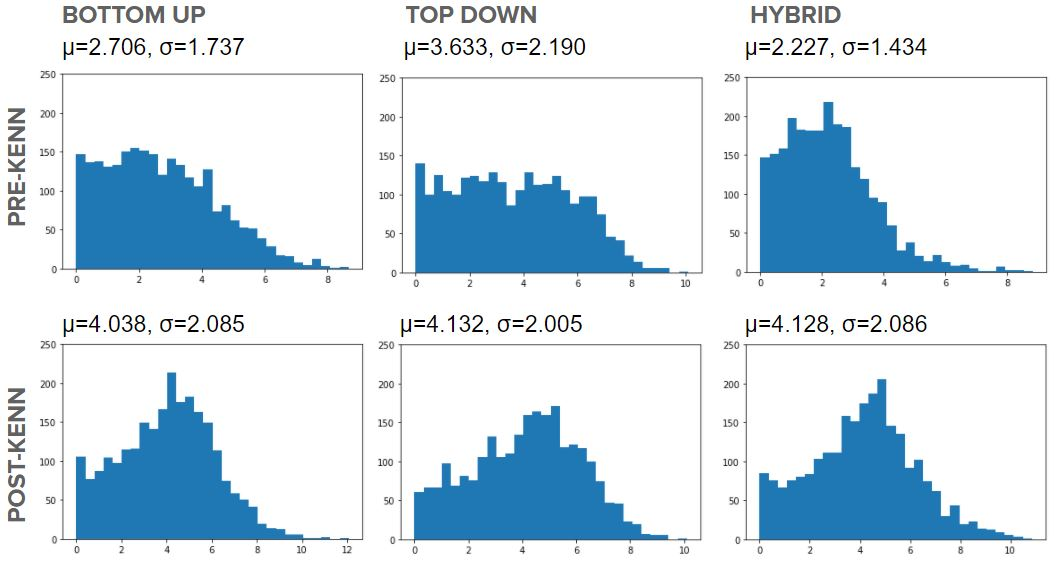
\includegraphics[scale=.53]{figures/kenn_pos_distrib.JPG}
    \caption{Distribution of the pre-KENN and post-KENN positive preactivations for each KB mode. Computed on the dev set of FIGER.}
    \label{fig:kenn_pos_distrib}
\end{figure}

\begin{figure}[H]
    \centering
    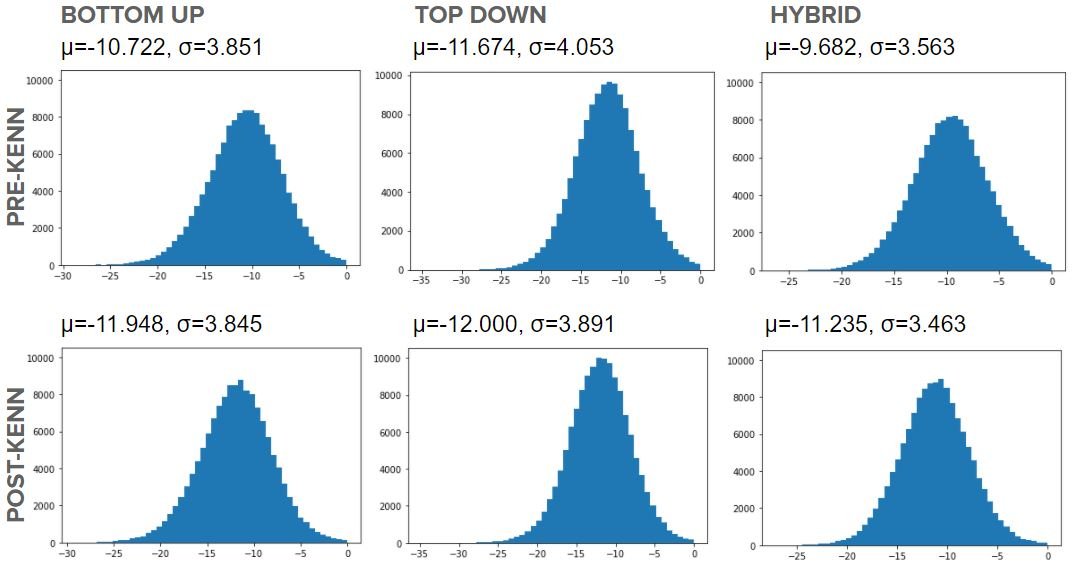
\includegraphics[scale=.53]{figures/kenn_neg_distrib.JPG}
    \caption{Distribution of the pre-KENN and post-KENN negative preactivations for each KB mode. Computed on the dev set of FIGER.}
    \label{fig:kenn_neg_distrib}
\end{figure}

\paragraphn{Preactivations analysis 2 and 3 - FSM and Sankey diagrams}
The analysis of the Finite State Machines and the Sankey diagrams can help to understand how the pre-KENN and post-KENN preactivations are modified depending on types F and S involved in the same clause, thus providing other insights into the suspicion of adaptation emerged in the previous study.

Starting from the Bottom Up mode, we can find the FSM and the Sankey diagram in Figure~\ref{fig:transitions_bottom_up}. We remind that a Bottom Up clause will always produce a positive delta on F and a negative delta on S. Indeed, F1S0 is a sink vertex of the Bottom Up FSM because F can never be decreased and S can never be increased in a Bottom Up setup. By analyzing the information of the transitions, we can observe that:
\begin{enumerate}
    \item The percentages of wrong transitions represent a minority.
    \item The probability of remaining in the forbidden state (i.e., F0S1) is 0.03. This is reasonable because the forbidden state represents also a clause violation (i.e., 1$\to$0) for this KB mode, so KENN will always try to modify the predictions to reach another post-KENN state. In these cases, the percentages of correctness show that the outgoing transitions from F0S1 never lead to worse predictions, but this is trivial since it is a wrong state by definition.
    \item The statistics about the transition F0S1$\to$F1S0 are quite counterintuitive since F and S are reversed correctly in 43.1\% of cases. The fact that the pre-KENN network predicts F as negative and S as positive when the target is the opposite is curious. It is plausible that the pre-KENN network learned that a type F usually receives one or more positive boosts, so it produces an initial negative prediction being aware that KENN will correct the final value. 
    \item The transition F0S0$\to$F1S0 could seem weird too. It has a probability of 0.01 and a percentage of correctness of 84.3\%. Some of these transitions are due to the fact that in the Bottom Up mode a type F is involved in multiple clauses, so the positive boost could derive from one or more siblings of S. However, after an investigation, it emerged that there are several examples of transitions F0S$_{1,...,n}$0$\to$F1S$_{1,...,n}$0 where F becomes positive thanks to the aggregated boost of its negative children. In particular, on a total of 500 F0S0$\to$F1S0 transitions, in 78 of them the effect of a single S was sufficient to enhance F. Even this behavior could be explained by the fact that the pre-KENN network learned that F is used to receive positive boosts.
\end{enumerate}


\begin{figure}
     \centering
     \begin{subfigure}{0.7\textwidth}
         \centering
         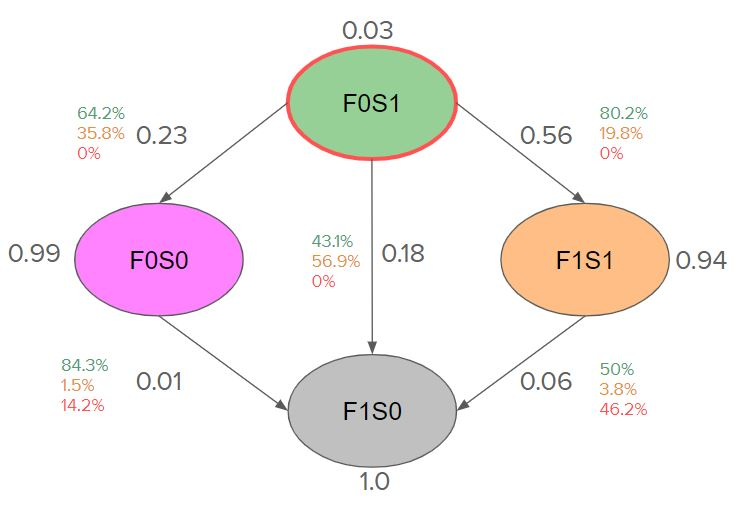
\includegraphics[width=\textwidth]{figures/fsm_bottom_up.JPG}
         \caption{FSM}
         \label{fig:fsm_bottom_up}
         \vspace{15px}
     \end{subfigure}
     \vfill
     \begin{subfigure}{0.6\textwidth}
         \centering
         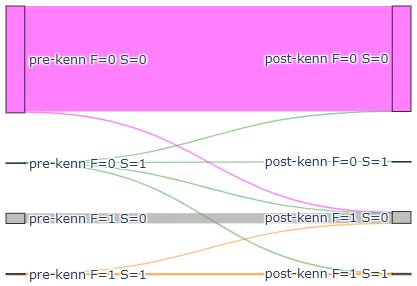
\includegraphics[width=\textwidth]{figures/sankey_bottom_up.JPG}
         \caption{Sankey diagram}
         \label{fig:sankey_bottom_up}
     \end{subfigure}
        \caption{FSM and Sankey diagram of the Bottom Up mode on the dev set of FIGER.}
        \label{fig:transitions_bottom_up}
\end{figure}

The FSM and the Sankey diagram of the Top Down mode are shown in Figure~\ref{fig:transitions_top_down}. The first thing we can notice is that the transitions of the FSM have opposite directions with respect to Bottom Up, so the sink vertex becomes F0S1. Looking at the statistics of the transitions, we can observe that:
\begin{enumerate}
    \item The percentages of wrong transitions represent a minority.
    \item The incoming transitions of the forbidden state have null probabilities when starting from F0S0 or F1S1, and near-zero probability when the pre-KENN state is F1S0. This is a very interesting fact, since it means that the pre-KENN network produces predictions such that KENN cannot generate a boost that leads to the forbidden state.
    \item Even if in this KB mode the pre-KENN state F1S0 may represent a clause violation (i.e., 1$\to 0 \vee ... \vee 0$) that KENN will try to correct, we can still find some examples of self-loop transition. Note that the high probability of 0.867 is due to the fact that in a Top Down clause the consequent is a disjunction of siblings. However, if we exclude from the count the cases in which a sibling of S is positive, we still have a high probability of 0.512 of self-loop. This means that the pre-KENN network learned to generate preactivations that prevent the effect of KENN when the desired output is F1S0.
    \item If we look at the Sankey diagram in Figure~\ref{fig:sankey_top_down}, we can see that the pre-KENN state F0S1 (i.e., the sink node) is missing. In this case too, the reason can be found in the fact that the pre-KENN network is aware that KENN will not be able to change the final predictions.
\end{enumerate}

\begin{figure}
     \centering
     \begin{subfigure}{0.7\textwidth}
         \centering
         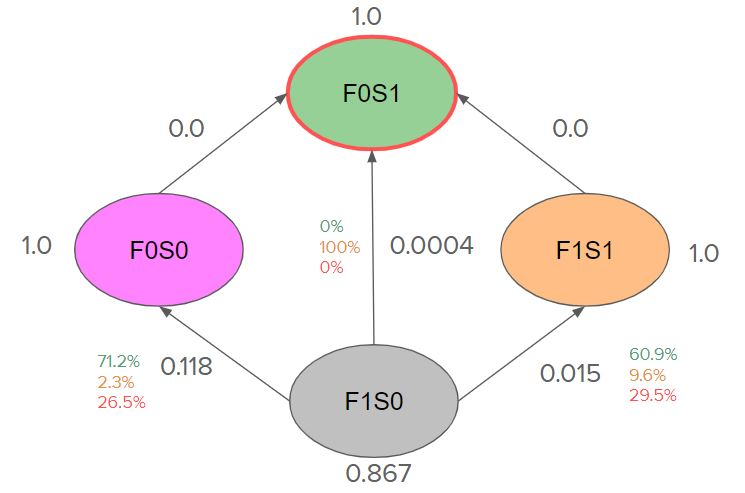
\includegraphics[width=\textwidth]{figures/fsm_top_down.JPG}
         \caption{FSM}
         \label{fig:fsm_top_down}
         \vspace{15px}
     \end{subfigure}
     \vfill
     \begin{subfigure}{0.6\textwidth}
         \centering
         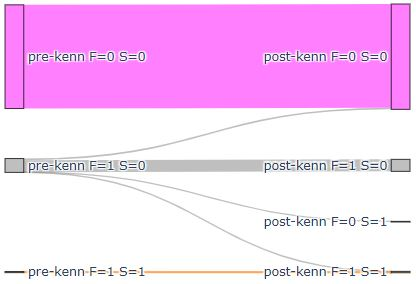
\includegraphics[width=\textwidth]{figures/sankey_top_down.JPG}
         \caption{Sankey diagram}
         \label{fig:sankey_top_down}
     \end{subfigure}
        \caption{FSM and Sankey diagram of the Top Down mode on the dev set of FIGER.}
        \label{fig:transitions_top_down}
\end{figure}

Finally, we can find the transitions of the Hybrid mode in Figure~\ref{fig:transitions_hybrid}. The FSM transitions are bidirectional because they are inherited from Top Down and Bottom Up. The consequence is that there are no sink nodes and all the transitions become potentially available. The considerations we can make by observing the figures are that:
\begin{enumerate}
    \item The percentages of wrong transitions represent a minority.
    \item Similarly to what happens in the Top Down, the probability to make a transition into the forbidden state is null.
    \item The probability of remaining in the forbidden state is very low like in the Bottom Up.
    \item The Sankey diagram is denser than those of Bottom Up and Top Down, since it is constituted by the mix of their transitions.
\end{enumerate}

\begin{figure}
     \centering
     \begin{subfigure}{0.7\textwidth}
         \centering
         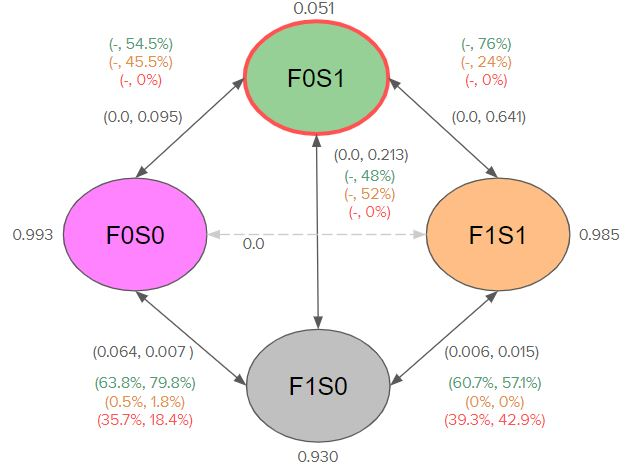
\includegraphics[width=\textwidth]{figures/fsm_hybrid.JPG}
         \caption{FSM - perecentages and probabilities are reported as \textit{(x, y)}, where \textit{x~=~value~of~down-to-up~transition} and \textit{y~=~value~of~up-to-down~transition}  }
         \label{fig:fsm_hybrid}
         \vspace{15px}
     \end{subfigure}
     \vfill
     \begin{subfigure}{0.6\textwidth}
         \centering
         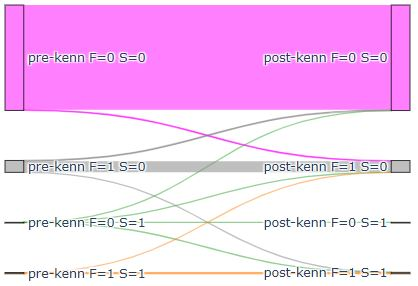
\includegraphics[width=\textwidth]{figures/sankey_hybrid.JPG}
         \caption{Sankey diagram}
         \label{fig:sankey_hybrid}
     \end{subfigure}
        \caption{FSM and Sankey diagram of the Hybrid mode on the dev set of FIGER.}
        \label{fig:transitions_hybrid}
\end{figure}

A final consideration can be done by comparing the three Sankey diagrams: even if their starting states are quite different, their final states become very similar. This fact is analogous to what we observed when comparing the pre-KENN and post-KENN preactivations.

\paragraphn{Preactivation analysis - Conclusion}
This study brought to light several aspects that confirmed the suspicion of adaptation. In the first analysis we saw that while the pre-KENN distributions had relevant differences, the post-KENN distributions became more similar to each other and to the baseline. We then detected other evident signals of adaptation by analyzing the transitions of the FSMs and the Sankey diagrams. Considering the Bottom Up mode, the most representative examples can be found in the transitions F0S1$\to$F1S0 and F0S0$\to$F1S0, where the pre-KENN network seems to be aware of the boost that will be produced on F by KENN. Even more interesting is the situation of the Top Down. Here, the strongest adaptation signals are given by the absence of F0S1 (i.e., sink node) as pre-KENN state in the Sankey diagram and by the high probability of not correcting a violated clause (i.e., self-loop on F1S0).